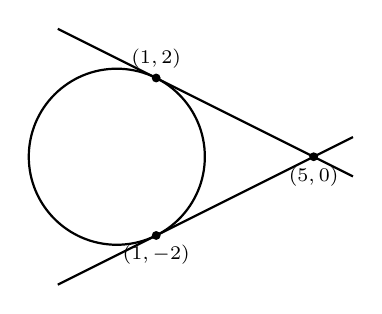
\begin{tikzpicture}[x=5mm,y=5mm]
\ax{-3}{6}{-3.5}{3.5}
\draw[thick,domain=-1.5:6,samples=80] plot (\x,{(5-\x)/2});
\draw[thick,domain=-1.5:6,samples=80] plot (\x,{(\x-5)/2});
\fill (5,0) circle (1.6pt);
\node[below] at (5,0){\scriptsize $(5,0)$};
\fill (1,2) circle (1.6pt);
\node[above] at (1,2){\scriptsize $(1,2)$};
\fill (1,-2) circle (1.6pt);
\node[below] at (1,-2){\scriptsize $(1,-2)$};
\draw[thick] (0,0) circle (2.236);
\end{tikzpicture}